\documentclass{beamer}

% Beamer style
\usetheme{CambridgeUS}
\usecolortheme[rgb={0.65,0.15,0.25}]{structure}
\beamertemplatenavigationsymbolsempty

% Packages
\usepackage[latin1]{inputenc}
\usepackage{color,graphicx}
\usepackage{url}
\usepackage{amsmath, amsfonts, amssymb}
\usepackage{/home/robin/LATEX/Biblio/astats}

% Commands
\definecolor{darkred}{rgb}{0.65,0.15,0.25}
\definecolor{darkgreen}{rgb}{0,0.4,0}
\newcommand{\emphase}[1]{{#1}}
\newcommand{\paragraph}[1]{\textcolor{darkred}{#1}}
\newcommand{\refer}[1]{\textcolor{gray}{\sl \cite{#1}}}
\newcommand{\Refer}[1]{\textcolor{gray}{\sl #1}}
\newcommand{\newblock}{}
\newcommand{\ra}{$\emphase{\rightarrow}$}

% Symbols


%====================================================================
\title[ABS4NGS]{ABS4NGS: Algorithmic, Bioinformatic and Software for Next
Generation Sequencing data}

\author[S. Robin]{AA Bioinformatics 2011 \\ ~\\
  Headed by E. Barillot, Institut Curie \\ ~\\
  INRA group: UMR 518 AgroParisTech / INRA MIA \\
  \bigskip \bigskip 
  \paragraph{Aims.} Develop, implement, validate and transfer powerful analysis methods for NGS: genome resequencing, RNA-Seq, ChIP-Seq, Methyl-Seq, Chromosome Conformation Capture (HiC) and Ori-Seq, \dots
}

\institute[AgroParisTech / INRA]{}

\date[February 2014]{INRA, February 2014}

%====================================================================

%====================================================================
%====================================================================
\begin{document}
%====================================================================
%====================================================================

%====================================================================
\frame{\titlepage
  }

% pr�sentation de l'IA et de ses objectifs 1 � 2 diapos
% gouvernance 1 diapo
% Etat d'avancement 1 diapo
% difficult�s rencontr�es et �ventuelles mesures correctives � prendre  1 diapo


%====================================================================
%====================================================================
\frame{\frametitle{Partners \& fundings}

  {%\footnotesize
  \begin{tabular}{p{.45\textwidth}p{.3\textwidth}cc} %p{.05\textwidth}p{.05\textwidth}}
  Partner & Expertise & kE & ETP \\
  \hline
  Curie/INSERM/CNRS Bioinfo \& Comp Syst Biol &  systems biology, \newline biostatistics & 520 & 66 \\ \hline
  Plateforme INCA Synergie Lyon Cancer & biology, NGS, \newline data management & 290 & 48 \\ \hline
  Curie/ARMines CBio & statistical learning & 243 & 28\\ \hline
  Agro/INRA - MIA & statistics, algorithmics & 241 & 58 \\ \hline
  Informatique Gaspard Monge & computer sciences, \newline algorithmics & 205 & 48 \\ \hline
  Biometrie et Biologie Evolutive & biology, statistics, \newline computer sciences & 309 & 44\\ \hline
  Genostar & software publisher & 189 & 60 \\
  \hline
  & +bioinformatics (all) & 2,000 & 352
  \end{tabular}
  }
  
% \begin{enumerate}
% \item U900 Institut Curie / INSERM / CNRS Bioinformatics and Computational Systems Biology: Systems biology, biostatistics
% \item Plateforme Inca Synergie Lyon Cancer: Biology, data management
% \item ARMINES / CBio: Statistical learning
% \item UMR 518 AgroParisTech / INRA - MIA: Statistics, algorithmics
% \item Laboratoire d'Informatique Gaspard Monge: Computer sciences, algorithmics
% \item Laboratoire de Biometrie et Biologie Evolutive: biology, statistics, computer sciences
% \item Genostar: software publisher
% \end{enumerate} 
% 
% \ra + bioinformatics expertise for all of them.

}

%====================================================================
\frame{\frametitle{General picture}
  $$
  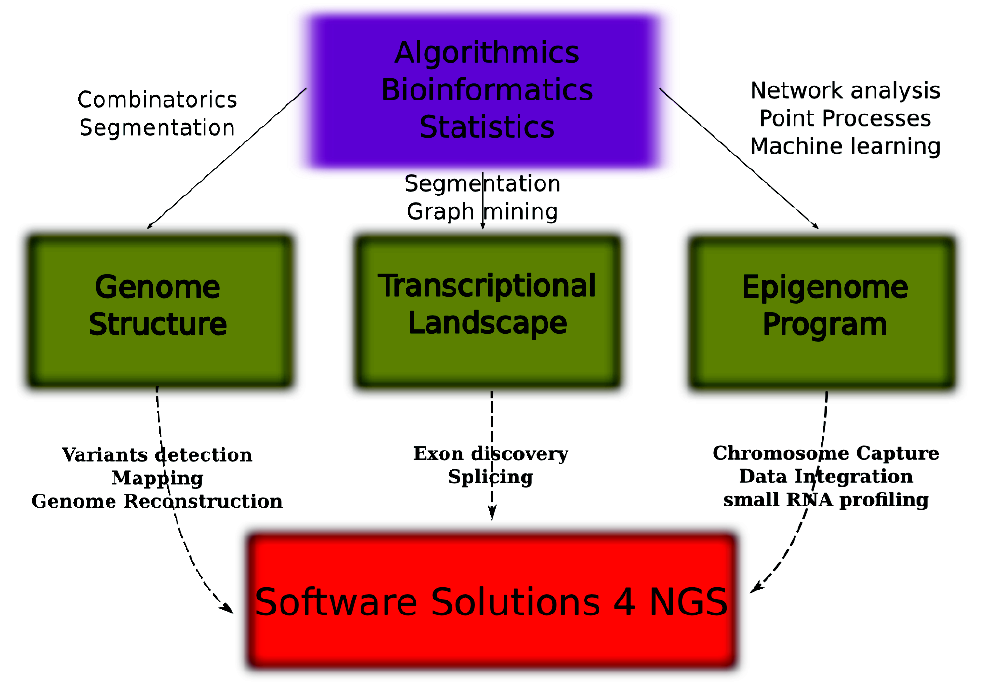
\includegraphics[width=.8\textwidth]{../Figures/ABS4NGS-Organigram}
  $$
  }
  
%====================================================================
\frame{\frametitle{Work-packages}

  \vspace{-0.02\textheight}
  \begin{tabular}{p{.35\textwidth}p{.55\textwidth}}
    From short reads to genome reconstruction & 
    {\footnotesize
	 Data, benchmark and validation \newline
	 Mapping NGS reads to a reference genome \newline
	 SNPs, point mutation \& small Indels detection \newline
	 Large size CNVs \& rearrangements 
	 } \\ \hline 
    Transcriptional landscape & 
    {\footnotesize
	 Gene expression analysis using annotation \newline
	 Re-annotation of transcribed regions \newline
	 Exon splicing
	 } \\ \hline 
    Epigenomics & 
    {\footnotesize
	 Chromatin and Chromosome Structural changes \newline
	 DNA Replication and Genome Organization \newline
	 Gene regulation from DNA modifications and DNA/Protein interactions \newline
% 	 Biological Models to investigate Gene Expression controls \newline
	 Probabilistic modeling of Sequencing Coverage \newline
	 Statistics for Differential Peak Identification
	 } \\ \hline 
    \multicolumn{2}{l}{Towards a software product}
  \end{tabular}

%   \begin{enumerate}
%    \item From short reads to genome reconstruction 
%    \begin{itemize}
%     \item Data, benchmark and validation
%     \item Mapping NGS reads to a reference genome
%     \item SNPs , point mutation & small Indels detection
%     \item Large size CNVs & rearrangements
%    \end{itemize}
%    \item Transcriptional landscape
%    \begin{itemize}
%     \item Gene expression analysis using annotation
%     \item Re-annotation of transcribed regions
%     \item Exon splicing
%    \end{itemize}
%    \item Epigenomics
%    \begin{itemize}
%     \item Chromatin and Chromosome Structural changes
%     \item DNA Replication and Genome Organization
%     \item Gene regulation from DNA modifications and DNA/Protein interactions
%     \item Biological Models to investigate Gene Expression controls
%     \item Probabilistic modeling of Sequencing Coverage
%     \item Statistical Methods for Differential Peak Identification
%    \end{itemize}
%    \item Towards a software product
%   \end{enumerate}

}

%====================================================================
\frame{\frametitle{Management}

  \paragraph{Headed by} E. Barillot, Institut Curie (P1)
  
  \bigskip
  \paragraph{Duration} 4 years
  
  \bigskip
  \paragraph{Website:}  \url{https://sites.google.com/site/abs4ngs/}
  
  \bigskip
  \paragraph{2 meetings a year:} Paris / Lyon / Paris
  
  \bigskip
  \paragraph{Scientific committee:} J-B Veyrieras (Biom�rieux), M. Brudno (univ. Toronto), S. Dudoit (univ. Berkeley), I. Gut (CN Analisis Genomico, Spain), J-J Codani (GenomeQuest)  \\
  \ra Visit during one of the 2014 meetings
  
}

%====================================================================
\frame{\frametitle{Some progresses}

  \paragraph{Bioinformatics} {\footnotesize
  \begin{itemize}
  \item Pipeline for the detection of somatic mutations
  \item Multi-factor normalization method for CNV in ultra-depth targeted sequencing
  \item ENU mutagenesis screening for the identification of new components of the piRNA pathway in mouse
  \item Bioinformatics developpments for ChIP-Seq
  \end{itemize}}
  
  \bigskip
  \paragraph{Algorithmics} {\footnotesize
  \begin{itemize}
  \item Dynamic indexing for accurate read mapping
  \end{itemize}}

  \bigskip
  \paragraph{Statistics} {\footnotesize
  \begin{itemize}
  \item Structure variation detection with correction to the GC-content and mappability
  \item Alternative splicing: Estimation of the relative abundance of isoforms
  \item Statistical comparison of transcript boundaries
  \item Statistical segmentation of HiC data
  \end{itemize}}
 
}

%====================================================================
\frame{\frametitle{Issues}

  Not too many up to now, except:
  \begin{itemize}
   \item Some delays for the signature of the consortium agreement.
   \item How to combine academic diffusion of GPL package and software publisher rights?
  \end{itemize}

}

%====================================================================
\frame{\frametitle{Oral}

  \paragraph{Interest for INRA}
%  Impact pour l'INRA (plus-value de la collaboration inter-�tablissements par rapport aux capacit�s propres � l'INRA)
  \begin{itemize}
  \item Access to very recent technologies (and associate problems), e.g. HiC
  \item Reinforcement of existing collaborations (Curie, LBBE, ...)
  \item New connexions with academic partners (G. Monge)
  \end{itemize}

  \bigskip\bigskip
  \paragraph{Interactions with other IA projects}
% Interactions en cours ou souhait�es entre projets IA, sur le plan organisationnel (partage d'exp�riences, partage d'outils) et sur le plan scientifique
  \begin{itemize}
   \item ABS4NGS aims at providing tools for the whole community interested in next generation sequencing technologies
   \item UMR 518 also involved in Amaizing: common methodologies to be used
  \end{itemize}

}


 


%====================================================================
%====================================================================
\section*{Appendix}
{\tiny
  \bibliography{../../../../Biblio/ARC,../../../../Biblio/AST,../../../../Biblio/SSB}
  \bibliographystyle{../../../../LATEX/astats}
  %\bibliographystyle{plain}
  }

%====================================================================
%====================================================================
\end{document}
%====================================================================
%====================================================================


\frame{\frametitle{}
  }

  \vspace{-0.5cm}
  \begin{tabular}{cc}
    \hspace{-0.5cm}
    \begin{tabular}{p{.5\textwidth}}
    \end{tabular}
    &
    \hspace{-1cm}
    \begin{tabular}{p{.5\textwidth}}
    \end{tabular}
  \end{tabular}
